% !TEX root = knauss-vissuelizer.tex
\section{Example Scenarios}
In this section we describe examples that highlight the functionality of the \viss tool.

\subsection{Where are the hotspots in a set of issues?}
Often, a clear understanding of requirements only evolves during the development of software.
This is especially true (but not limited to) agile software projects, where managers decide to frame only rudimentary requirements and refine the details on the go.
For a manager, it is important to know when problematic requirements surface, because they can have a serious impact on the project.
\viss helps managers in this scenario as follows:
\begin{enumerate}
\item The manager loads a set of issues (e.g. user stories for the current iteration).
\item \viss automatically analyzes the comments that are related to these issues and that are available in online communication.  
\item \viss creates a set of \emph{clarification trajectories} (c.f. Figure \ref{fig:example-trajectory}), one for each issue. 
Comments that are concerned with clarifying requirements are depicted by red rectangles below the timeline, other comments are depicted by blue rectangles above the timeline.
\item \viss also displays suggestive pattern names for distinctive trajectories (e.g. textbook-example, back-to-draft, procrastination).
\item The manager scrolls through the issues and associated trajectories and decides based on this rich information where to invest more resources.
\end{enumerate}
\begin{figure}
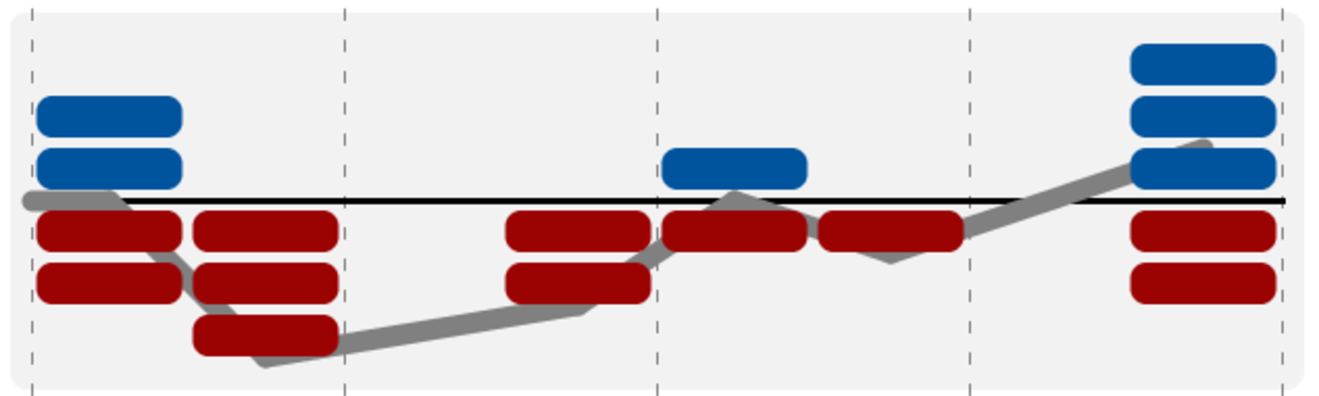
\includegraphics[width=\columnwidth]{img/example-trajectory}
\caption{Example of a clarification trajectory}
\label{fig:example-trajectory}
\end{figure}
Typically, there is a number of issues without pathological findings, e.g. user stories with some clarification in the beginning and other communication events later on that show progress. But there are also suspicious trajectories: a large amount of clarification late in the iteration, perhaps even after the issue seemed to be solved. 
Or no clarification at all, even though the issue seems to be complex.

\subsection{Are there any communication breakdowns?}
After identifying those hotspots, the manager most likely wants to continue with a closer investigation. 
Often, he or she will investigate who participates in a discussion of an issue and who is not.
\viss helps managers in this scenario by creating social networks for an issue or a set of issues on the fly.
More over, \viss also integrates information of the automatic analysis of online communication into these social networks, i.e. showing for each actor the percentage of clarification and other communication.
Figure \ref{fig:example-sn} shows an example of an social network for the issue presented in Figure \ref{fig:example-trajectory}. 
\begin{figure}
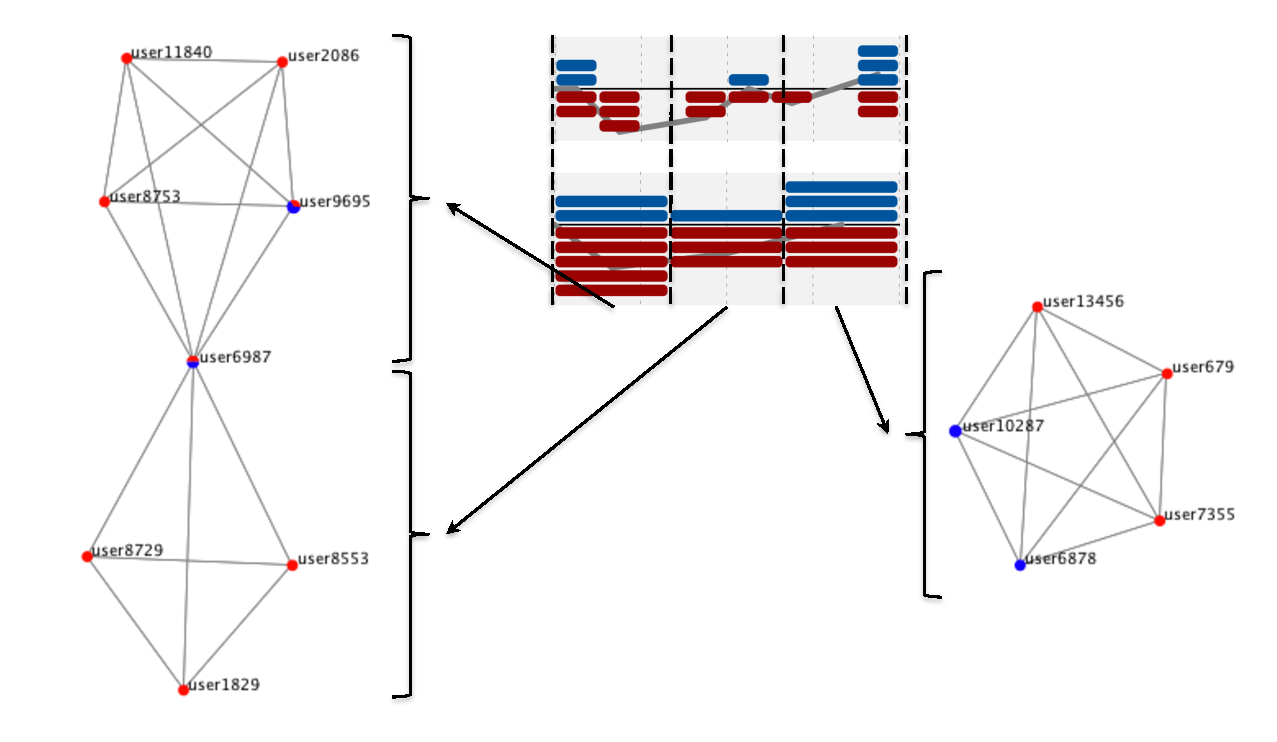
\includegraphics[width=\columnwidth]{img/example-sn}
\caption{Example of a social network}
\label{fig:example-sn}
\end{figure}
The developers are presented as nodes (here: anonymized), and connections between nodes are weighted by the amount of communication both developers share about a given issue in a specific time interval. 
In the example above, the manager might conclude that there is no single person who is coordinating the work around this issue, because there is no actor who participates in all relevant time intervals.
A suitable action might be to assign the responsibility to a more experienced developer.

\subsection{Who is knowledgeable about a given topic?}

Integrating the right persons in the loop for an important feature is a crucial ability for managers.
To support managers in this task, \viss distinguishes between two types of knowledge: domain knowledge that shows in communication events related to clarification and technical knowledge that shows in other communication events.
In order to leverage the power of \viss for this task, the manager selects a number of issues that are related to a given topic. 
\viss integrates the social networks of these issues in a single large network (see Figure \ref{fig:example-sn-large}).
\begin{figure}
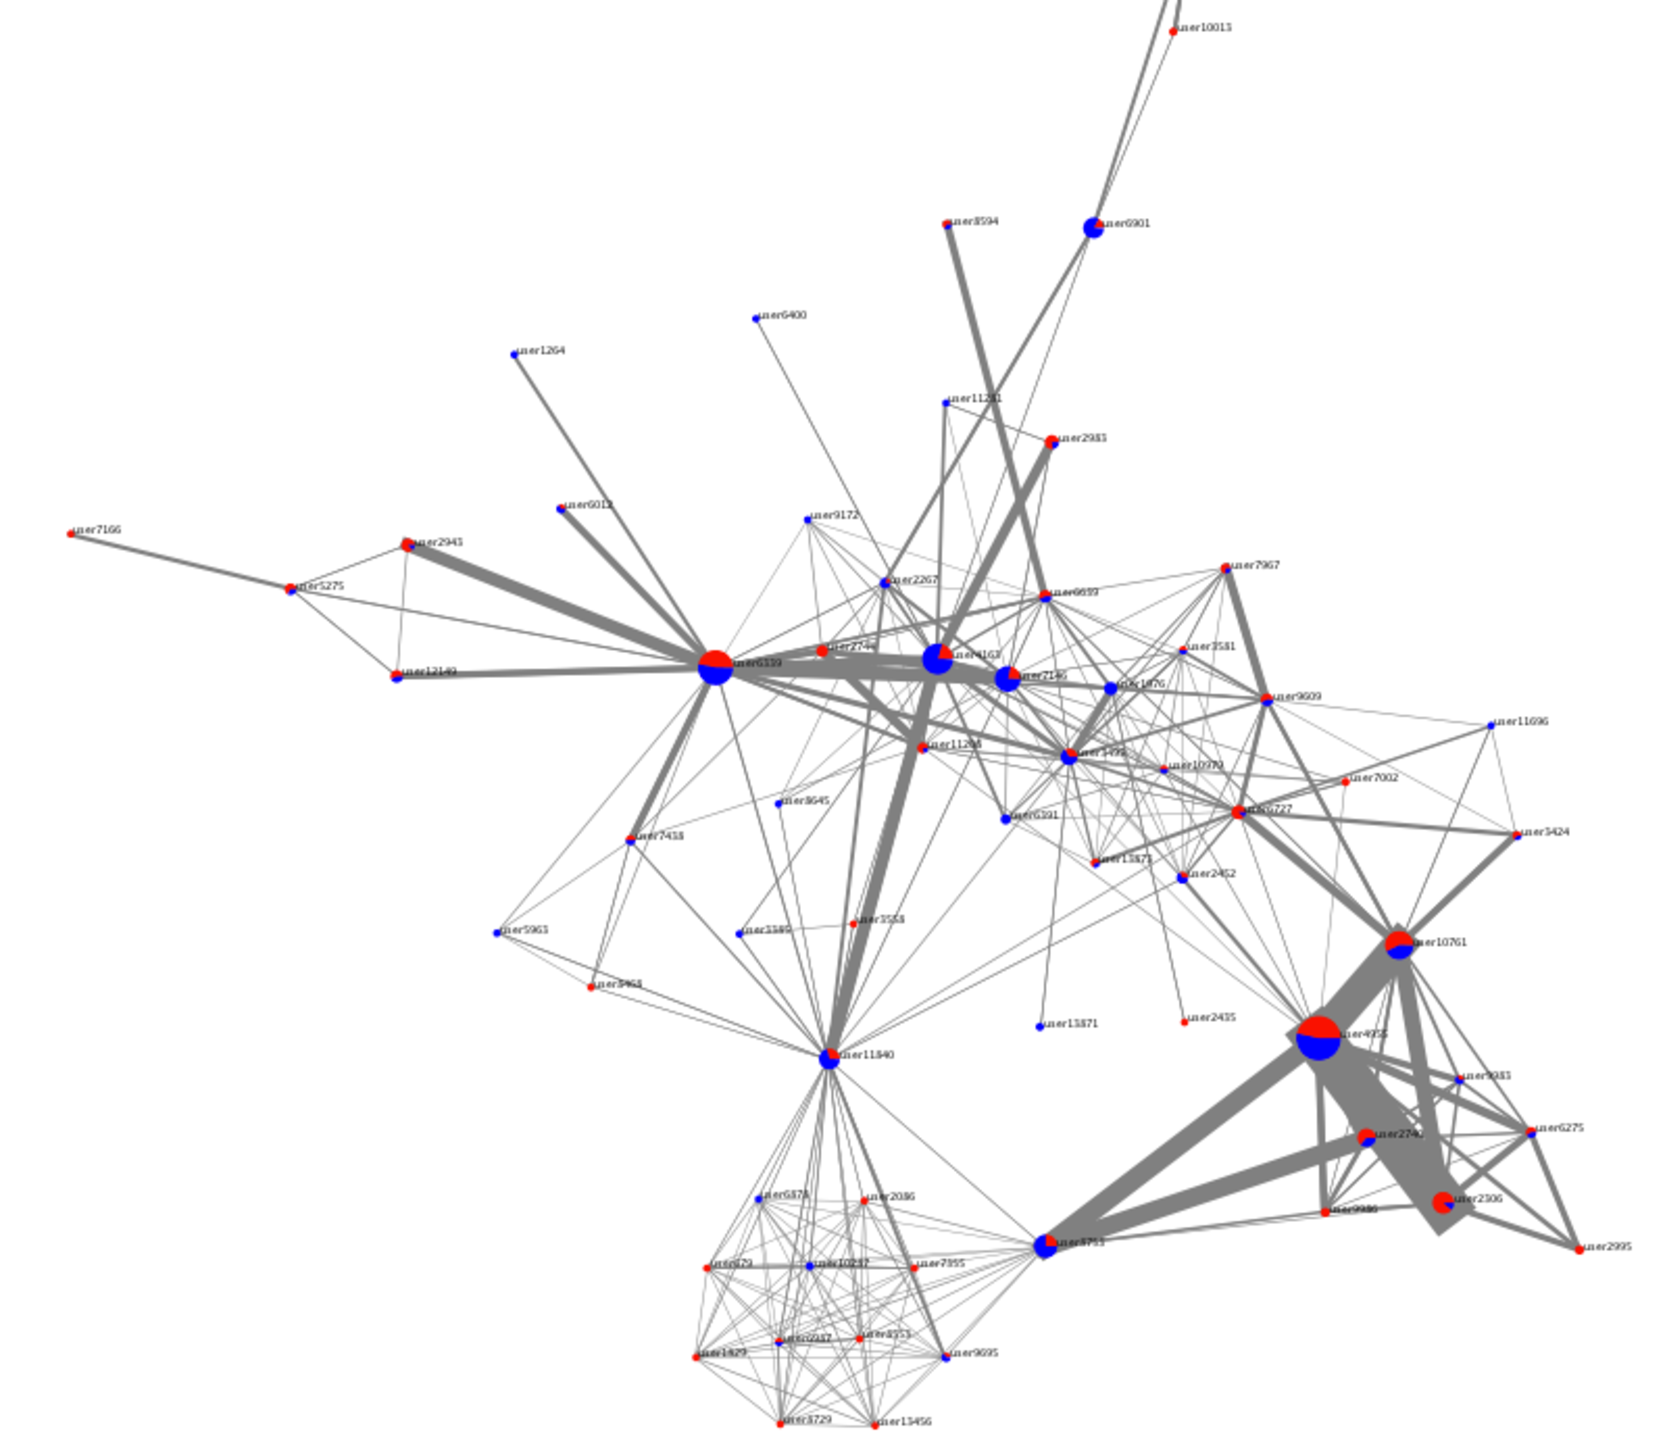
\includegraphics[width=\columnwidth]{img/example-sn-large}
\caption{Example of a social network of a set of issues}
\label{fig:example-sn-large}
\end{figure}
The manager looks for candidates with a balanced percentage of clarification and other communication and a medium centrality, actors with high centrality might already have a very high workload.
